\documentclass[10.5pt,a4paper]{article}
\usepackage[a4paper,top=0.9in,bottom=0.9in,left=0.9in,right=0.9in]{geometry}
\usepackage[T1]{fontenc}
\usepackage[utf8]{inputenc}
\usepackage{lmodern}
\usepackage{xcolor}
\usepackage{graphicx}
\usepackage{listings}
\usepackage{booktabs}
\usepackage{enumitem}
\usepackage{hyperref}
\usepackage{titlesec}
\usepackage{fancyhdr}
\usepackage{microtype}
\usepackage{parskip}
\usepackage{amsmath}

\definecolor{accent}{HTML}{1F6F78}
\definecolor{codebg}{HTML}{F4F6F8}
\definecolor{codeframe}{HTML}{D9DEE4}
\definecolor{muted}{HTML}{5B6472}

\hypersetup{colorlinks=true, linkcolor=accent, urlcolor=accent, citecolor=accent}

\titleformat{\section}{\normalfont\Large\bfseries\color{black}}{\thesection}{0.6em}{}
\titleformat{\subsection}{\normalfont\large\bfseries\color{black}}{\thesubsection}{0.5em}{}
\titlespacing*{\section}{0pt}{1.4em}{0.7em}
\titlespacing*{\subsection}{0pt}{1.1em}{0.5em}

\pagestyle{fancy}
\fancyhf{}
\renewcommand{\headrulewidth}{0.4pt}
\fancyhead[L]{\small\color{muted}Delhivery Hub Reliability \& SLA Study}
\fancyhead[R]{\small\color{muted}Technical Report}
\fancyfoot[C]{\small\color{muted}\thepage}

\lstdefinestyle{py}{
  backgroundcolor=\color{codebg},
  rulecolor=\color{codeframe},
  frame=single,
  framesep=6pt,
  basicstyle=\ttfamily\footnotesize,
  keywordstyle=\color{accent}\bfseries,
  commentstyle=\color{muted}\itshape,
  stringstyle=\color{teal},
  numbers=left,
  numberstyle=\tiny\color{muted},
  numbersep=8pt,
  breaklines=true,
  language=Python,
  showstringspaces=false,
  xleftmargin=1em,
  xrightmargin=0.2em,
}
\lstset{style=py}

\title{\vspace{-2em}\textbf{\Large Delhivery Hub Reliability \& SLA Simulation}\\[0.3em]
\large\color{muted} Does fleet size or SLA design drive on-time delivery?}
\author{Jnanadyuti Patra}
\date{September 2026}

\begin{document}
\maketitle
\vspace{-2em}

\noindent
\textbf{Code \& data:} \url{https://github.com/Jnanadyuti-Patra/delhivery-hub-reliability-sim}\\
\textbf{Live dashboard:} \url{https://jnanadyuti-patra.github.io/delhivery-hub-reliability-sim/}

\vspace{1em}
\hrule
\vspace{1em}

\section{Problem Statement}

Delhivery, one of India's largest integrated logistics providers, dispatches shipments from hub to hub across the country. Like any delivery network, it sometimes misses its delivery promise. There are two structurally different explanations for a missed service-level agreement (SLA), and each implies a different fix:

\begin{enumerate}[leftmargin=1.4em]
  \item \textbf{A capacity problem.} If shipments are delayed because they are queued waiting for an available vehicle, the fix is operational: add more vehicles to the dispatch fleet.
  \item \textbf{A promise-design problem.} If vehicles are freely available but individual trip times are inherently variable (traffic, weather, road conditions, distance), then adding vehicles does nothing --- the fleet was never the bottleneck. The fix here is to set a more realistic delivery promise, or to change \emph{how} shipments are routed, not how many vehicles carry them.

\end{enumerate}

This report documents a discrete-event simulation built on Delhivery's own real operational data to distinguish between these two explanations for one real hub, and to turn the answer into a concrete, quantified recommendation.

\section{Data}

The dataset is Delhivery's public operational release: \textbf{144,867 real GPS/scan records}, covering trips across Indian cities and states between 12 September and 6 October 2018. Row count and field structure were verified against the documented public dataset before use.

Each shipment is tracked through a \texttt{trip\_uuid}, moving through one or more \texttt{source\_center} $\rightarrow$ \texttt{destination\_center} legs. For every leg, the data records:

\begin{itemize}[leftmargin=1.4em]
  \item \texttt{route\_type}: \textbf{Carting} (smaller, typically local pickup/delivery runs) or \textbf{FTL} --- Full Truck Load (one truck dedicated to a single shipment, typically longer routes).
  \item \texttt{actual\_time}: the real, observed transit time for that leg (minutes).
  \item \texttt{osrm\_time}: the transit time predicted by OSRM, an open-source routing engine --- effectively the ``map estimate,'' analogous to a Google Maps ETA.
  \item \texttt{osrm\_distance}: the routing engine's planned distance for the leg (km).
\end{itemize}

A shipment is scanned at multiple checkpoints as it moves, which means a single leg between two centers can appear as several rows with increasing cumulative \texttt{actual\_time}/\texttt{osrm\_time} values. The cleaning step below collapses these into one real observation per leg.

\section{Methodology}

No machine learning model was trained for this study. The problem being asked --- \emph{``if we changed the fleet size or the routing policy, what would happen?''} --- is a counterfactual, causal question about a system's operating mechanics, not a pattern-recognition question about historical correlations. A predictive ML model (e.g.\ a regression predicting delivery time from features) would only tell us what \emph{already happened} under the fleet size and policies actually used historically; it cannot tell us what would happen under a fleet size or policy that was never tried. \textbf{Discrete-event simulation (DES)} was chosen instead, because it lets us directly rebuild the mechanism --- vehicles, queues, dispatch --- and then run it under hypothetical conditions that never occurred in the real data.

\subsection{Step 1 --- Cleaning the Real Data}

\texttt{src/01\_clean\_data.py} collapses the repeated checkpoint scans for each (\texttt{trip\_uuid}, \texttt{source\_center}, \texttt{destination\_center}) leg down to one final observation, using the \emph{maximum} cumulative \texttt{actual\_time} / \texttt{osrm\_time} recorded for that leg (the last checkpoint before the shipment moved on):

\begin{lstlisting}
grp = df.groupby(["trip_uuid", "source_center", "destination_center"],
                  as_index=False).agg(
    route_type=("route_type", "first"),
    actual_time=("actual_time", "max"),
    osrm_time=("osrm_time", "max"),
    osrm_distance=("osrm_distance", "max"),
    ...
)
grp["delay_ratio"] = grp["actual_time"] / grp["osrm_time"]
\end{lstlisting}

This produced \textbf{26,003 clean trip legs} across \textbf{1,487 source hubs} nationally, each with a real \texttt{delay\_ratio} --- how many times longer the trip actually took versus what the routing engine predicted.

\subsection{Step 2 --- The Simulation Model}

\texttt{src/02\_simulate\_hub\_policy.py} models outbound dispatch at \textbf{Gurgaon\_Bilaspur\_HB}, the busiest source hub in the dataset (1,062 legs), restricted to its \textbf{Medium-distance tier} (77--299\,km) --- the one tier where both Carting and FTL are genuinely used side by side in the real data, making it the actual decision point a dispatcher faces.

The simulation is built with \textbf{SimPy}, a Python discrete-event simulation library. Two features of the real world are modeled explicitly:

\begin{itemize}[leftmargin=1.4em]
  \item \textbf{A limited vehicle pool}, represented as a \texttt{simpy.Resource}. A new shipment must acquire a vehicle before it can depart; if all vehicles are busy, it queues, exactly as it would at a real dispatch yard.
  \item \textbf{Bootstrapped real timing}, not a fitted theoretical distribution. Instead of assuming transit times follow (say) a Normal or Exponential curve, every simulated trip's \texttt{(actual\_time, osrm\_time)} pair is drawn \emph{with replacement} directly from the real historical legs of that route type. This preserves the true, messy relationship between planned and actual time, including its long right tail.
\end{itemize}

\begin{lstlisting}
def dispatch_proc(dispatch_id):
    ready_time = env.now
    rt = "Carting" if rng.random() < hist_carting_share else "FTL" \
         if policy == "Historical" else policy
    actual_time, osrm_time = draw_leg(rng, rt)   # real bootstrapped pair
    with fleet.request() as req:
        yield req                                # wait for a free vehicle
        wait = env.now - ready_time
        yield env.timeout(actual_time)            # occupy it for the real trip time
        total_time = env.now - ready_time
        on_time = total_time <= SLA_BUFFER * osrm_time
        log.append((rt, wait, actual_time, osrm_time, total_time, on_time))
\end{lstlisting}

Dispatches themselves arrive following the real historical \emph{interarrival gaps} observed at this hub and tier --- also bootstrapped, so simulated traffic is as bursty (or as calm) as the real hub actually was. The simulation is run for 150 independent replications per scenario (each a simulated 30-day month) to average out sampling noise.

\subsection{Step 3 --- Experiment 1: Is It a Fleet-Size Problem?}

With the SLA promise fixed at 2$\times$ the OSRM-planned time (close to the $\sim$2.1--2.5$\times$ average delay observed nationally), the outbound fleet size was swept from 2 to 24 vehicles, under three routing policies: all-Carting, all-FTL, and the real historical 55\%/45\% Carting/FTL mix. For every combination, on-time rate and average dispatch wait time were recorded.

\subsection{Step 4 --- Experiment 2: What SLA Can Each Policy Actually Deliver?}

\texttt{src/03\_sla\_buffer\_sweep.py} follows directly from Experiment 1's finding (Section 4). With fleet size fixed at 12 vehicles --- a level at which queueing wait is already effectively zero --- the \emph{SLA buffer itself} was swept from 1.5$\times$ to 5$\times$ the planned time, to find the tightest delivery promise each routing policy can hit 90\% of the time.

\section{Results}

\subsection{The raw pattern: real deliveries run well past the plan}

\begin{figure}[h!]
  \centering
  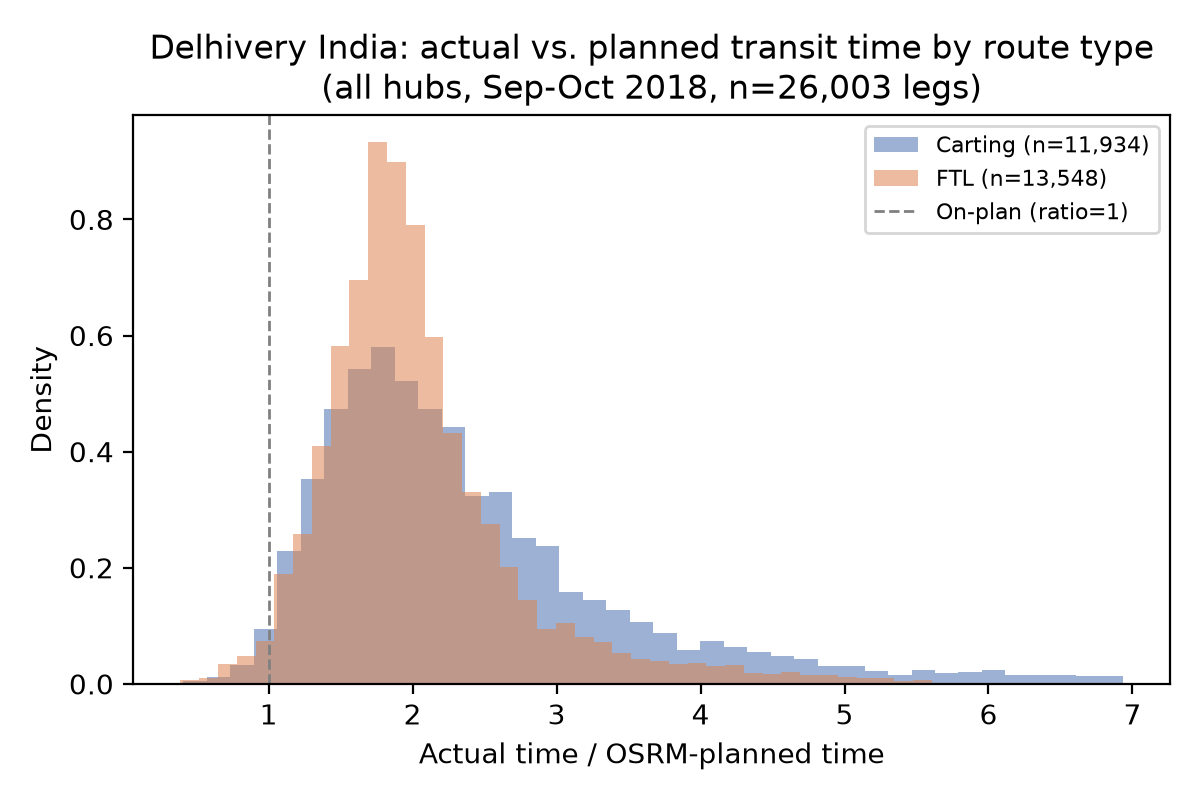
\includegraphics[width=0.85\textwidth]{../output/01_delay_ratio_distribution.png}
  \caption{Actual-to-planned transit time ratio, all 26,003 legs nationally. A ratio of 1.0 means the delivery took exactly as long as the routing engine predicted. Carting averages 2.51$\times$ the plan; FTL averages 2.15$\times$.}
\end{figure}

\begin{figure}[h!]
  \centering
  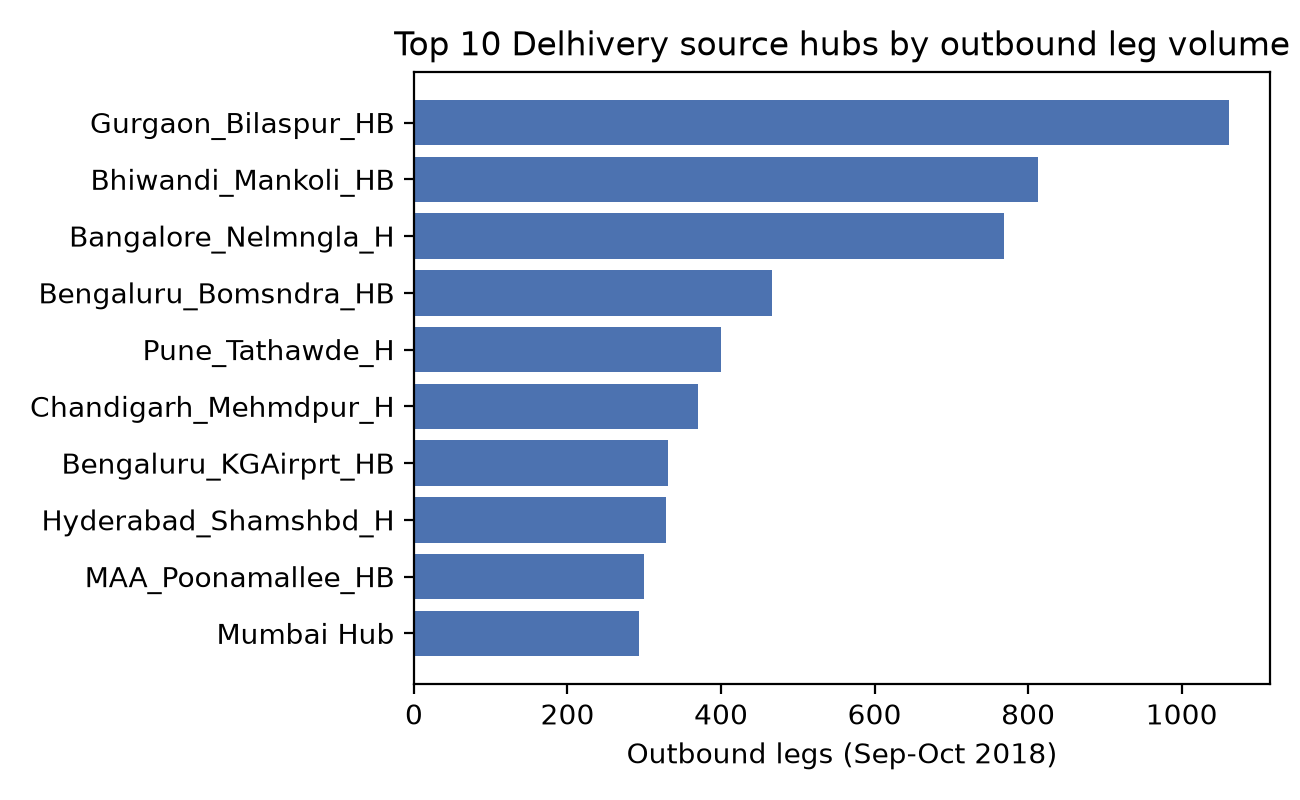
\includegraphics[width=0.75\textwidth]{../output/00_top_hubs.png}
  \caption{Gurgaon\_Bilaspur\_HB is the single busiest outbound hub in the dataset, making it the natural hub to model in depth.}
\end{figure}

\clearpage
\subsection{Experiment 1: fleet size is not the bottleneck}

\begin{figure}[h!]
  \centering
  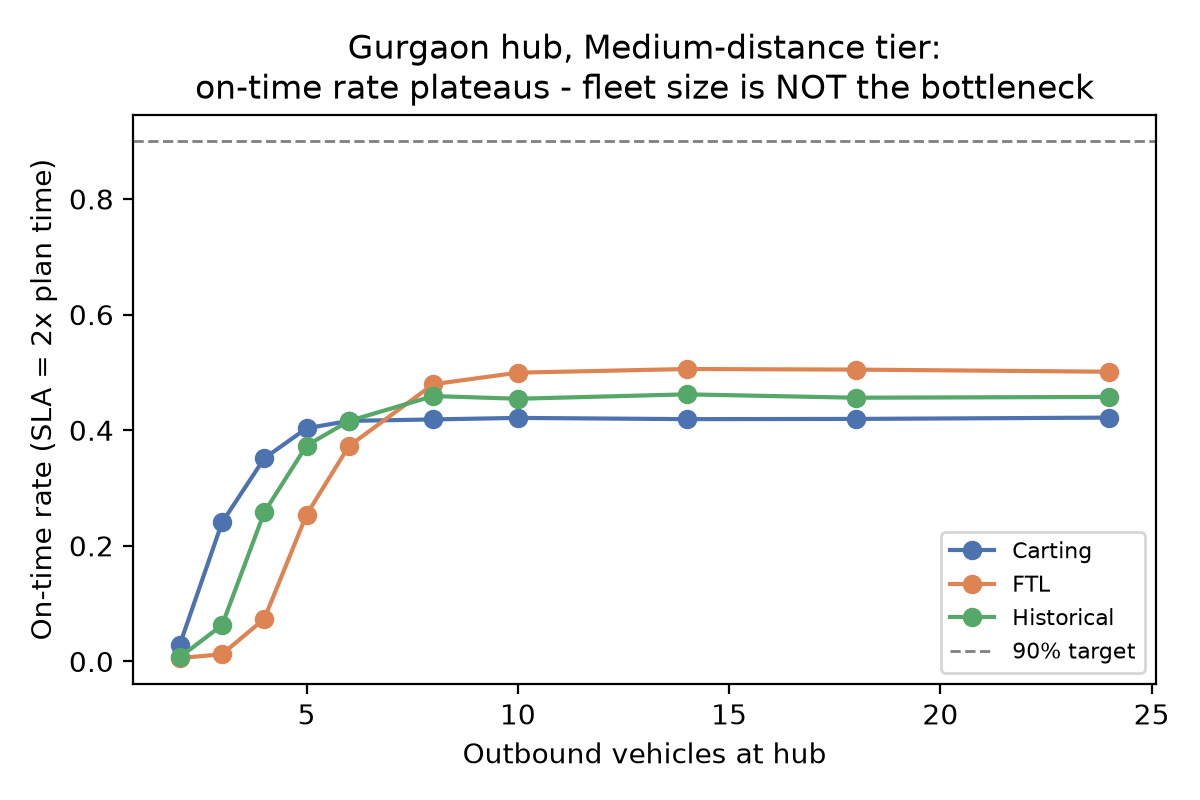
\includegraphics[width=0.85\textwidth]{../output/02_fleet_size_vs_ontime.png}
  \caption{On-time rate vs.\ outbound fleet size, at a fixed 2$\times$ SLA. By $\sim$8 vehicles, average dispatch wait time is already near zero (the queue has emptied) --- yet on-time rate plateaus at only 42--50\%. Adding more vehicles beyond this point changes nothing.}
\end{figure}

\textbf{Finding:} this rules out Explanation 1 from Section 1. The hub is not capacity-constrained at this SLA target; the ceiling on on-time performance comes from the inherent variability of individual trip times, not from vehicles sitting idle in a queue.

\subsection{Experiment 2: the real lever is routing policy and SLA design}

\begin{figure}[h!]
  \centering
  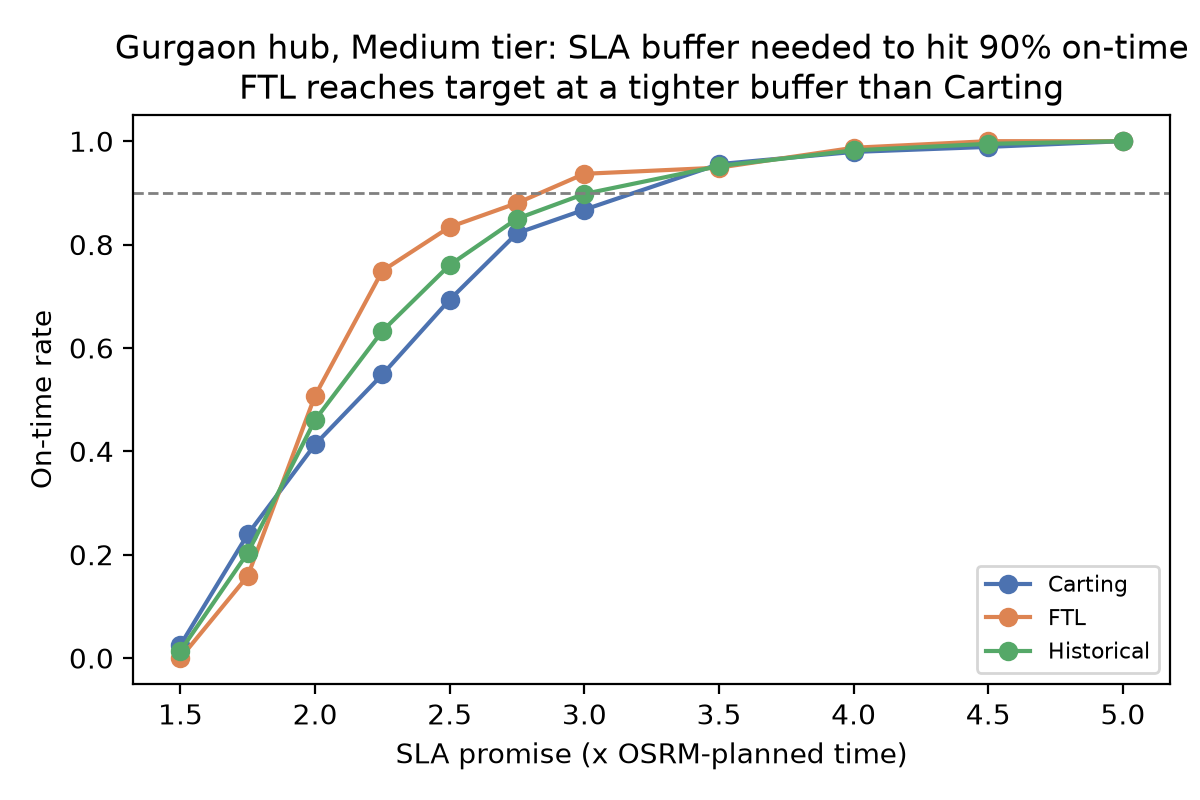
\includegraphics[width=0.85\textwidth]{../output/03_sla_buffer_vs_ontime.png}
  \caption{On-time rate vs.\ SLA buffer (fleet size fixed at 12, congestion-free). FTL reaches the 90\% target at a tighter buffer than Carting or the historical mix.}
\end{figure}

\begin{table}[h!]
\centering
\begin{tabular}{@{}lccc@{}}
\toprule
\textbf{Policy} & \textbf{Min.\ buffer for 90\% on-time} & \textbf{Avg.\ delay ratio (national)} & \textbf{Historical share} \\
\midrule
FTL             & \textbf{3.0$\times$ plan time} & 2.15$\times$ & 45\% \\
Historical mix  & 3.5$\times$ plan time & --- & --- \\
Carting         & 3.5$\times$ plan time & 2.51$\times$ & 55\% \\
\bottomrule
\end{tabular}
\caption{SLA buffer required to hit a 90\% on-time rate, by routing policy, Gurgaon hub, Medium-distance tier.}
\end{table}

\section{Recommendation}

For Medium-distance corridors out of the Gurgaon hub, routing shipments via \textbf{FTL} instead of Carting (or the current historical mix) lets the hub promise a \textbf{tighter, shorter delivery window} (3.0$\times$ the routing engine's planned time, versus 3.5$\times$) while holding the same 90\% reliability target. This is a zero-capital-expenditure recommendation --- no new vehicles required --- driven purely by which routing policy is used for this tier.

\section{Limitations}

\begin{itemize}[leftmargin=1.4em]
  \item The dataset carries no fare or freight-cost field. Vehicle-hours consumed (not currency) was used as the operational-efficiency proxy throughout; a real per-trip cost model would let this recommendation be stated in rupees saved, not just buffer-time tightened.
  \item The analysis is scoped to one hub (Gurgaon\_Bilaspur\_HB) and one distance tier (Medium, 77--299\,km), the tier with the clearest real-world overlap between Carting and FTL usage. Other hubs or tiers may show different dynamics.
  \item The dataset spans roughly three weeks (12 Sep -- 6 Oct 2018); seasonal effects (festival traffic, monsoon disruption) are not represented.
\end{itemize}

\section{Reproducibility}

The full pipeline --- data cleaning, both simulation experiments, and the chart-generation script --- is published with documentation at:
\url{https://github.com/Jnanadyuti-Patra/delhivery-hub-reliability-sim}. An interactive results dashboard is live at:
\url{https://jnanadyuti-patra.github.io/delhivery-hub-reliability-sim/}.

\end{document}
